\section{Background and Motivation}\label{sec:background}

This section builds up the problem this paper addresses.
% 本节建立本文要解决的问题。
Section~\ref{sec:pipeline} describes the pipeline that takes an eBPF program from writing to execution, Section~\ref{sec:need} shows why the effect of an optimization depends on the machine that loads the program, and Section~\ref{sec:whynot} presents the two obstacles that have kept per-machine rewriting from happening.
% 2.1 节描述 eBPF 程序从编写到执行的流水线,2.2 节说明优化的效果为何取决于装载程序的机器,2.3 节说明为每台机器改写程序至今未能实现的两个障碍。

\subsection{The eBPF Pipeline}\label{sec:pipeline}

An eBPF program passes through a fixed pipeline from writing to execution, and Figure~\ref{fig:pipeline} shows the whole of it.
% 一个 eBPF 程序从编写到执行经过一条固定的流水线,图 1 展示它的全貌。
Developers write the program in restricted C and compile it on a build machine into portable bytecode.
% 开发者用受限的 C 语言编写程序,在构建机上编译成可移植的字节码。
At load time, the kernel rewrites the places in the bytecode that depend on kernel data layout to match the layout of the target kernel, a step that only lets the program access data correctly and performs no optimization~\cite{llvm-bpf-reloc}.
% 装载时,内核把字节码中依赖内核数据布局的位置按目标内核的实际布局改写,这一步只让程序正确地访问数据,不做任何优化。
Once the program passes verification, the in-kernel just-in-time compiler lowers the bytecode to machine code, and the result attaches to a fixed attachment point of the kernel called a~hook.
% 通过验证之后,字节码由内核中的即时编译器译成机器码,挂到内核预设的挂载点上运行。

\begin{figure}[t]
\centering
% 图:eBPF 流水线。视觉词汇:工件=白框,执行组件=蓝色填充框,动作=箭头标签(distribute、load);
% 目标机器内部虚线横隔线分 user space 与 kernel 两带,带标签在框外左侧,证明图例填入 user space 带右侧空当;
% 阴影罩字节码与验证器(证明覆盖范围),JIT 与机器码在阴影外。所有框同尺寸,间距一致。
% 自带库声明与缩放,保证不依赖主文件导言区也能编译且不溢出栏宽。
\usetikzlibrary{arrows.meta,positioning,fit,backgrounds,calc}
\resizebox{\columnwidth}{!}{%
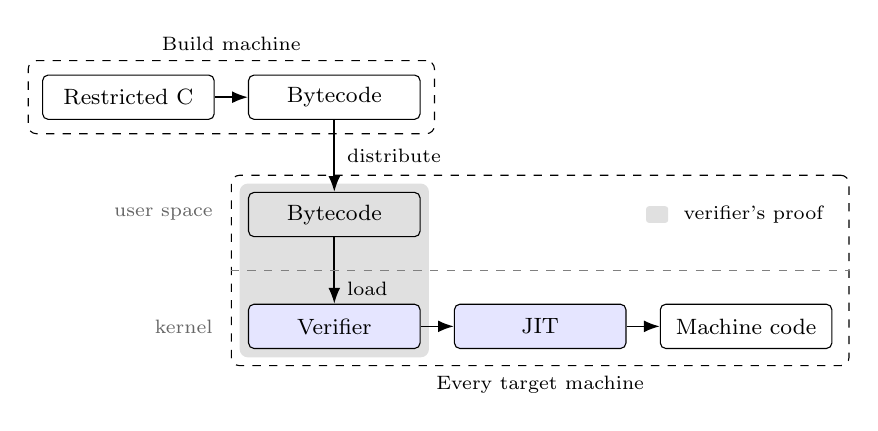
\begin{tikzpicture}[
  box/.style={draw, rounded corners=2pt, font=\footnotesize, minimum width=6.2em, minimum height=1.6em, inner sep=2pt},
  mach/.style={box, fill=blue!10},
  lbl/.style={font=\scriptsize},
  dim/.style={font=\scriptsize, text=black!60},
  arrow/.style={-Latex, semithick}
]
% 目标机器,kernel 带(下行)
\node[mach] (verif) {Verifier};
\node[mach, right=1.2em of verif] (jit) {JIT};
\node[box, right=1.2em of jit] (native) {Machine code};
% 目标机器,user space 带(中行)
\node[box, above=2.4em of verif] (byte2) {Bytecode};
% 构建机(上行)
\node[box, above=2.6em of byte2] (byte) {Bytecode};
\node[box, left=1.2em of byte] (src) {Restricted C};
% 箭头
\draw[arrow] (src) -- (byte);
\draw[arrow] (byte) -- node[lbl, right=1pt]{distribute} (byte2);
\draw[arrow] (byte2) -- node[lbl, right=1pt, pos=0.78]{load} (verif);
\draw[arrow] (verif) -- (jit);
\draw[arrow] (jit) -- (native);
% 组框
\node[draw, dashed, rounded corners=3pt, inner sep=5pt, fit=(src)(byte),
      label={[lbl]above:Build machine}] (bm) {};
\node[draw, dashed, rounded corners=3pt, inner sep=6pt, fit=(byte2)(verif)(native),
      label={[lbl]below:Every target machine}] (tm) {};
% user space 与 kernel 的分界线与带标签
\coordinate (mid) at ($(byte2.south)!0.5!(verif.north)$);
\draw[dashed, black!50, thin] (tm.west |- mid) -- (tm.east |- mid);
\node[dim, anchor=east] at ([xshift=-3pt]tm.west |- byte2.center) {user space};
\node[dim, anchor=east] at ([xshift=-3pt]tm.west |- verif.center) {kernel};
% 证明覆盖阴影(罩字节码与验证器)
\begin{scope}[on background layer]
\fill[black!12, rounded corners=3pt]
  ([xshift=-3pt,yshift=-3pt]verif.south west) rectangle ([xshift=3pt,yshift=3pt]byte2.north east);
\end{scope}
% 图例,填入 user space 带右侧空当
\node[lbl, anchor=east] (plab) at ([xshift=-6pt]tm.east |- byte2.center) {verifier's proof};
\fill[black!12, rounded corners=1pt]
  ([xshift=-10pt,yshift=-3pt]plab.west) rectangle ([xshift=-2pt,yshift=3pt]plab.west);
\end{tikzpicture}%
}

\caption{The eBPF pipeline. The shaded region is what the verifier's proof covers, and the JIT output lies outside it.}
% 图:eBPF 的流水线。阴影是验证器证明的覆盖范围,JIT 的输出在其外。
\label{fig:pipeline}
\end{figure}

Before the verifier admits a program, it establishes what constrains the execution of that program.
% 验证器放行一个程序之前,会确认这个程序的执行受到哪些约束。
It requires every memory access to fall within bounds, requires the use of the stack to be bounded, and caps the number of instructions~\cite{gershuni2019simple,linuxkernel-bpf-verifier}.
% 它要求每次内存访问落在界内,要求栈的使用有界,并对指令数设上限。
Early verifiers admitted no loop at all, since Linux 5.3 they admit bounded loops that can be unrolled, and the newer interfaces leave the trip count to run time, where a cap applies only during execution.
% 早期的验证器不接受任何循环,自 Linux 5.3 起它接受可以被展开的有界循环,而更新的接口把循环次数交给运行时,只在执行时受上限约束。
Termination therefore holds for every program that can be loaded, whereas a static bound on the number of execution paths holds only for the programs that use no such loop.
% 因此,程序会终止这一条对所有可装载的程序成立,而执行路径条数有静态上界这一条,只对不含这类循环的程序成立。

The kernel functionality a program can reach is a catalog that can be listed entry by entry.
% 程序能够触碰的内核功能是一份可以逐条列出的清单。
A program calls kernel functions of two kinds, helpers with fixed numbers, whose prototypes live in the user-facing header of the kernel and from which the kernel's own script generates a machine-readable version, and kfuncs exported by symbol name, whose prototypes live in the type information of the kernel and carry no guarantee of stability across versions~\cite{gbadamosi2024ebpf}.
% 程序可以调用两类内核函数,一类是固定编号的 helper,其原型写在内核的用户接口头文件中,并由内核自带的脚本生成机器可读的版本,另一类是以符号名导出的 kfunc,其原型记录在内核的类型信息中,不保证跨版本稳定。
A program keeps state and exchanges data with user-space tools through shared tables called maps.
% 程序通过称为 map 的共享表保存状态并与用户态工具交换数据。
Beyond these two kinds of functions, the maps, and the context that the hook supplies, a program cannot reach the rest of the~system.
% 除这两类函数、map 与挂载点提供的上下文之外,程序无法触及系统的其余部分。

\subsection{The Machine-Dependence of an Optimization's Effect}\label{sec:need}

An eBPF program is optimized once on the build machine, and the effect of that optimization is decided by the machine that loads the program.
% 一个 eBPF 程序的优化在构建机上一次做完,而这次优化的效果由装载程序的那台机器决定。
The code is compiled and optimized before it is distributed to all machines, the rewriting at load time settles data layout alone, and the just-in-time compiler translates one instruction at a time without any optimization that depends on the processor model.
% 代码编译并优化之后分发到所有机器,装载时的改写只解决数据布局,即时编译器逐条翻译且不做依赖处理器型号的优化。
Differences between machines therefore never reach the code that finally executes, while they do reach the effect of executing that code.
% 机器之间的差别因此进不了最终执行的代码,却进得了这段代码的执行效果。

Instruction-by-instruction translation leaves a large gap, and closing it takes information that only the target machine holds.
% 逐条翻译留下的空间很大,而填补这段空间需要机器上的信息。
A measurement study of production applications finds that a hot memory-copy routine the compiler emits runs about ten times slower than the native implementation of the kernel on one machine~\cite{shahinfar2025demystifying}.
% 一项针对生产应用的测量研究发现,即时编译器译出的热点内存拷贝,在一台机器上比内核原生的实现慢约十倍。
The same study reports that the gain of one optimization varies with the workload and with the hook the program attaches to~\cite{shahinfar2025demystifying}.
% 同一项研究还报告,同一处优化的收益随负载与程序挂载的钩子而变。
At build time neither the machine that will load the program nor the workload it will face is known, and both are available only at run time on the~target~machine.
% 构建时既不知道程序会落在哪台机器上,也不知道它会面对什么负载,这些信息只在运行时的目标机器上才有。

Applying one fixed set of optimizations to all applications measures no faster than changing nothing at all.
% 把一套固定的优化施加到全部应用,测出的加速并不比什么都不改更大。
Table~\ref{tab:sameday} reports four conditions run on the same day under the same tasks and workloads, where each number is the ratio of the optimized to the baseline average run time per execution and a value below one means faster.
% 表 1 给出同一天在相同任务与负载下完成的四种条件,表中数值是优化后与基线的每次执行平均耗时之比,小于 1 表示更快。
The no-change control reads 0.954, the uniform mixed policy reads 0.997, the policy of K2 reads 0.982, and the policy of Merlin reads between 0.998 and 1.004~\cite{xu2021synthesizing,mao2024merlin}.
% 无改动的对照读出 0.954,统一施加的混合策略读出 0.997,K2 的策略读出 0.982,Merlin 的策略读出 0.998 到 1.004。
None of the four reads faster than the control, so one fixed set of optimizations cannot serve every machine, and serving each machine calls for rewriting the program for that machine.
% 四者之中没有一个快过对照,固定一套优化因此服务不了所有机器,要让每台机器都得到收益,就得为每台机器分别改写程序。

% 表:2026-06-27 同日四条件对比,x86 KVM,六应用固定负载,数值为逐会话几何平均后的总体几何平均。
%   数据出处 code/corpus/results/x86_kvm_corpus_20260627_*,按程序名配对、保留阈值 100 次执行。
%   noop 0.954(7 会话)、mixed 0.997(7)、k2 0.982(11)、merlin 1.004(7,区间 0.998-1.004)。
\begin{table}[t]
\footnotesize
\centering
\caption{Four conditions measured on the same day under the same tasks and workloads. A value below one means faster than the baseline phase of the same session.}
% 表:同一天在相同任务与负载下测得的四种条件。数值小于 1 表示快于同一会话的基线阶段。
\label{tab:sameday}
\begin{tabular}{llr}
\hline
Condition & What it applies & Run-time ratio \\
\hline
No-change control & nothing & 0.954 \\
Uniform policy & mixed bytecode passes & 0.997 \\
K2 policy & search-based rewrites~\cite{xu2021synthesizing} & 0.982 \\
Merlin policy & compile-time passes~\cite{mao2024merlin} & 1.004 \\
\hline
\end{tabular}
\end{table}


\subsection{Obstacles to Per-Machine Rewriting}\label{sec:whynot}

Rewriting a program for each machine requires two questions to be answered, whether the rewrite is in fact faster and whether the rewrite is still correct, and a live kernel makes both hard to answer.
% 为每台机器分别改写程序,要求回答两个问题,改写之后是否真的更快,以及改写之后是否仍然正确,而这两个问题在活内核上都难以回答。
The first question calls for measurement, and measurement on a kernel drifts.
% 前一个问题要靠测量,而内核上的测量本身会漂移。
The second question calls for a check, and the checks available today do not give the guarantee a rewrite needs.
% 后一个问题要靠检查,而今天可用的检查手段给不出改写所需的保证。

Measuring the same program twice on the same machine reads faster the second time.
% 同一个程序在同一台机器上先后测两次,第二次读出的速度更快。
The statistics switch of the kernel records the execution count and the accumulated run time of each program, which makes per-program measurement possible, and the baseline phase of a session and the phase that follows it run inside one boot, by which time the caches have warmed and the state of the kernel has changed.
% 内核的统计开关记录每个程序的执行次数与累计运行时长,逐程序的测量因此成为可能,而一次会话的基线阶段与其后的阶段在同一次启动之内先后进行,到后一个阶段,缓存已经变热,内核的状态也已改变。
We ran two controls that change nothing, one re-translating every program unchanged and one skipping the re-translation, and the two read 0.90 and 0.86, an apparent speedup of 10 to 14\% with nothing changed, measured on an earlier corpus of seven applications.
% 我们跑了两种什么都不改的对照,一种把每个程序原样重新翻译一遍,一种连重新翻译都跳过,二者分别读出 0.90 与 0.86,即什么都不改也有 10% 到 14% 的表观提速,这两个数字测自较早的、含七个应用的语料。
The no-change control of the batch in Table~\ref{tab:sameday} reads 0.954, so the size of the drift varies from batch to batch and a control has to run alongside the measured runs, and Figure~\ref{fig:noise} shows what these controls read.
% 表 1 那批的无改动对照读出 0.954,漂移的幅度因此随批次而变,对照必须与被测运行同期进行,图 2 展示这些对照读出的分布。
Programs executed fewer than about one hundred times also fluctuate far more widely than programs executed often, and programs entered through tail calls bypass the counting entry altogether, so the set of programs that takes part in a comparison has to be fixed in~advance.
% 此外,执行次数少于约一百次的程序,其读数的波动远大于执行次数多的程序,经尾调用进入的程序则绕过计数的入口,参与比较的程序集合因此需要事先划定。

\begin{figure}[t]
\centering
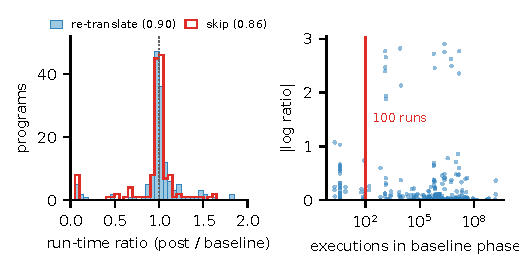
\includegraphics[width=\columnwidth]{figures/sec-2-noise-floor.pdf}
\caption{Left, the apparent per-program speedups read out by the two no-change controls. Right, the fluctuation of each program against its execution count.}
% 图:左,两种无改动对照读出的逐程序表观加速比;右,每程序的波动随执行次数的变化。
\label{fig:noise}
\end{figure}

Whether a rewrite is still correct is answered today by people and by tests, and neither gives the guarantee that a rewrite needs.
% 改写是否仍然正确,今天靠人与测试来回答,而两者都给不出所需的保证。
Practice is to maintain one program variant per kernel version, and a study of eBPF optimization observed exactly that in Tetragon while taking its measurements~\cite{mao2024merlin}.
% 工程上的做法是为每个内核版本各维护一份程序变体,一项对 eBPF 优化的研究在测量时观察到 Tetragon 正是如此。
Those variants are written by people and guarded by tests, yet a test can only sample inputs, and passing the tests does not mean agreeing with the original program on every input.
% 这些变体由人写成,把关靠测试,而测试只能抽取有限的输入,通过测试不等于在所有输入上都与原程序一致。
The rewritten code runs inside the kernel with no protection layer beneath it, so one error is not one failed process but a halt of the whole machine that takes the measuring process with it, and auditing after the fact is therefore not available on a kernel.
% 改写的代码运行在内核里,内核之下没有别的防护层,一次错误不是一个进程出错,而是整台机器停止,负责测量的进程随之消失,事后审查因此在内核上不成立。
Automatic eBPF optimizers take the other road and keep their rewrites correct by construction, at the cost of fixing the transformations they may apply before deployment, and Section~\ref{sec:related} sets out how those systems relate to this work.
% 自动的 eBPF 优化器换了另一条路,靠自身的构造保住正确性,代价是可以做的变换在部署前就已固定,第 6 节详述这些工作与本文的关系。